% ****************************************************************************************************
% Chapter 10: Explainability and Regulation
% ****************************************************************************************************

\chapter{Explainability and Regulation}
\label{ch:explainability}

A machine learning model that performs well is not, by itself, a machine learning model that can be deployed in a hospital. Before a system like mine can legally operate in an emergency department in the European Union after August 2026, it must satisfy a cluster of regulatory requirements that did not exist when most published medical ML was developed. Those requirements include transparency about how the model reaches its predictions, risk management in how errors are handled, data governance including explicit bias auditing, and human oversight structures that let a clinician understand, and when necessary override, the model's decisions.

This chapter brings those regulatory requirements together with the technical analysis that supports them. The central technique is SHAP, a method for attributing a model's prediction to its input features, which I use to examine both the model's global feature-importance pattern and its reasoning on individual patients. I discuss what SHAP shows, what it hides, and where the reasoning becomes uncomfortable. Then I turn to the regulatory framework: the European Union's Artificial Intelligence Act, specifically its treatment of emergency medical triage as high-risk AI, and what the statute requires of deployed systems. The chapter closes with a mapping of my work to the specific articles of the regulation.

The honest conclusion is that my system does some things well and others only partially. I present the picture as it is.

\section{Why Explainability Matters}

The question ``why did the model say ESI-2?'' is not academic. When a triage prediction is delivered to a nurse through a clinical decision-support interface, the nurse must decide whether to accept it. That decision is informed by a combination of the predicted level, any confidence or uncertainty information, and, in principle, some explanation of what features drove the prediction. A nurse who sees ``ESI-2, confidence 82\%'' without context is being asked to trust a black box. A nurse who sees ``ESI-2, confidence 82\%, driven primarily by an abnormal respiratory rate and a chief complaint flagged as similar to known cardiac cases'' has something to engage with: they can verify the respiratory rate independently, assess whether the cardiac comparison is apt, and decide whether to accept or override the prediction.

Explainability thus serves at least three distinct purposes. It supports informed clinical judgement at the point of use. It enables retrospective audit: when the model errs, explanations help diagnose \emph{why} it erred, which is necessary for continuous improvement. And it serves accountability: a patient, a regulator, or an adverse-event review panel can in principle inspect the model's reasoning on a specific case. The European Union's AI Act, which I discuss below, treats all three of these purposes as requirements, not options.

\begin{notebox}[What Is SHAP, Intuitively?]
SHAP (\emph{SHapley Additive exPlanations}) is a method for attributing a model's prediction to its input features. For each patient, it answers the question: how much did each feature contribute to the specific prediction the model made?

The name comes from cooperative game theory. Lloyd Shapley showed in 1953 that there is a unique way to fairly allocate credit among a team of cooperating players, satisfying four natural axioms (efficiency, symmetry, dummy, linearity). SHAP applies this mathematical machinery to machine learning: the ``players'' are the features, the ``game'' is producing a prediction, and the SHAP value for a feature is how much that feature contributed to moving the prediction away from the average prediction across the training set.

For tree-based models like mine, the specialised TreeSHAP algorithm computes these values exactly in polynomial time, which is why SHAP has become the standard explainability tool for gradient-boosted trees. The alternative for non-tree models (KernelSHAP) is slower and approximate.

What SHAP produces, for each patient, is a vector of feature-level contributions that sum to the final prediction minus the average prediction. Large positive contributions pushed the prediction toward the output; large negative contributions pushed against it. Summary statistics across many patients (mean absolute SHAP values) give global feature importance.
\end{notebox}

\section{The SHAP Setup, Honestly Described}

Before I present findings, I need to be precise about what was actually computed.

TreeSHAP operates on a single tree ensemble, not on a blend. My production model is a convex blend of five gradient-boosted tree models (Chapter~\ref{ch:architecture}); SHAP cannot be computed directly on the blend. The standard workaround is to compute SHAP on a representative single model, accepting that the attributions approximate the blend's behaviour rather than exactly describing it. I chose the baseline LightGBM member of the blend, trained on fold 5 of my stratified cross-validation split, with $200$ estimators. This model's out-of-fold macro F1 is $0.556$, compared to the full blend's $0.597$. The attributions I report should be read as approximately correct for the blend, with the caveat that the blend may weight features somewhat differently.

TreeSHAP was then run on a stratified random subsample of 20,000 patients drawn from the full 418,100-visit cohort, with stratification on the ESI label to ensure adequate representation of rare classes like ESI-1 and ESI-5. The resulting SHAP array has shape $(20000, 115, 5)$: one attribution for each of 20,000 patients, 115 features, and 5 acuity classes. The values are in log-odds space, LightGBM's native output for multiclass classification, rather than probability space. A SHAP value of $+1.0$ means that feature pushed the log-odds for that class up by one, which corresponds to a factor-of-$e$ increase in the odds ratio. This matters for reading waterfall plots: the same SHAP magnitude has a different visual meaning near the extremes of the probability range than near 0.5.

No SHAP interaction values were computed. TreeSHAP supports an interaction-value computation that breaks down each pair of features' joint contribution, but this was omitted from my production run due to memory constraints on the CPU compute node. The analysis in this chapter therefore cannot speak to how specific features interact; I discuss the features' individual contributions only. I flag this as a limitation: a deployed system subject to regulatory audit would likely be expected to report feature interactions on at least a sample of cases.

\begin{remarkbox}[Limitations of SHAP Itself]
SHAP is the current standard for tree-model explainability, but it is not a complete solution. Its axioms are satisfied in an aggregate sense, across all possible feature coalitions, but the individual SHAP values for a particular patient are a weighted summary rather than a causal explanation. A SHAP value of $+1.5$ for ``heart rate'' on a specific patient does not mean that ``raising the heart rate by one unit would raise the predicted log-odds by 1.5.'' It means that, averaging over all possible coalitions of other features being present or absent, the heart rate's marginal contribution on this patient was $1.5$.

For clinical interpretation, this subtlety matters. SHAP is better read as ``here is which features are most influential on this prediction'' than as ``here is what changed the prediction compared to a counterfactual.'' The latter question, counterfactual explanation, is a related but distinct technical problem that I do not address here.

Recent literature has also documented specific failure modes for SHAP, particularly around highly correlated features where multiple features capture similar signal and SHAP splits credit among them in ways that are mathematically correct but clinically confusing. My embedding features (emb\_pca\_0 through emb\_pca\_49) are all PCA components of the same underlying vector, so they are necessarily correlated, and the SHAP values for them should be interpreted as a group rather than individually.
\end{remarkbox}

\section{Global Feature Importance}

Figure~\ref{fig:shap-global} shows the mean absolute SHAP value across all 20,000 patients and all 5 classes for the top 20 features. This is the summary measure of ``how much, in aggregate, does this feature matter to the model's predictions?''

\begin{figure}[htbp]
 \centering
 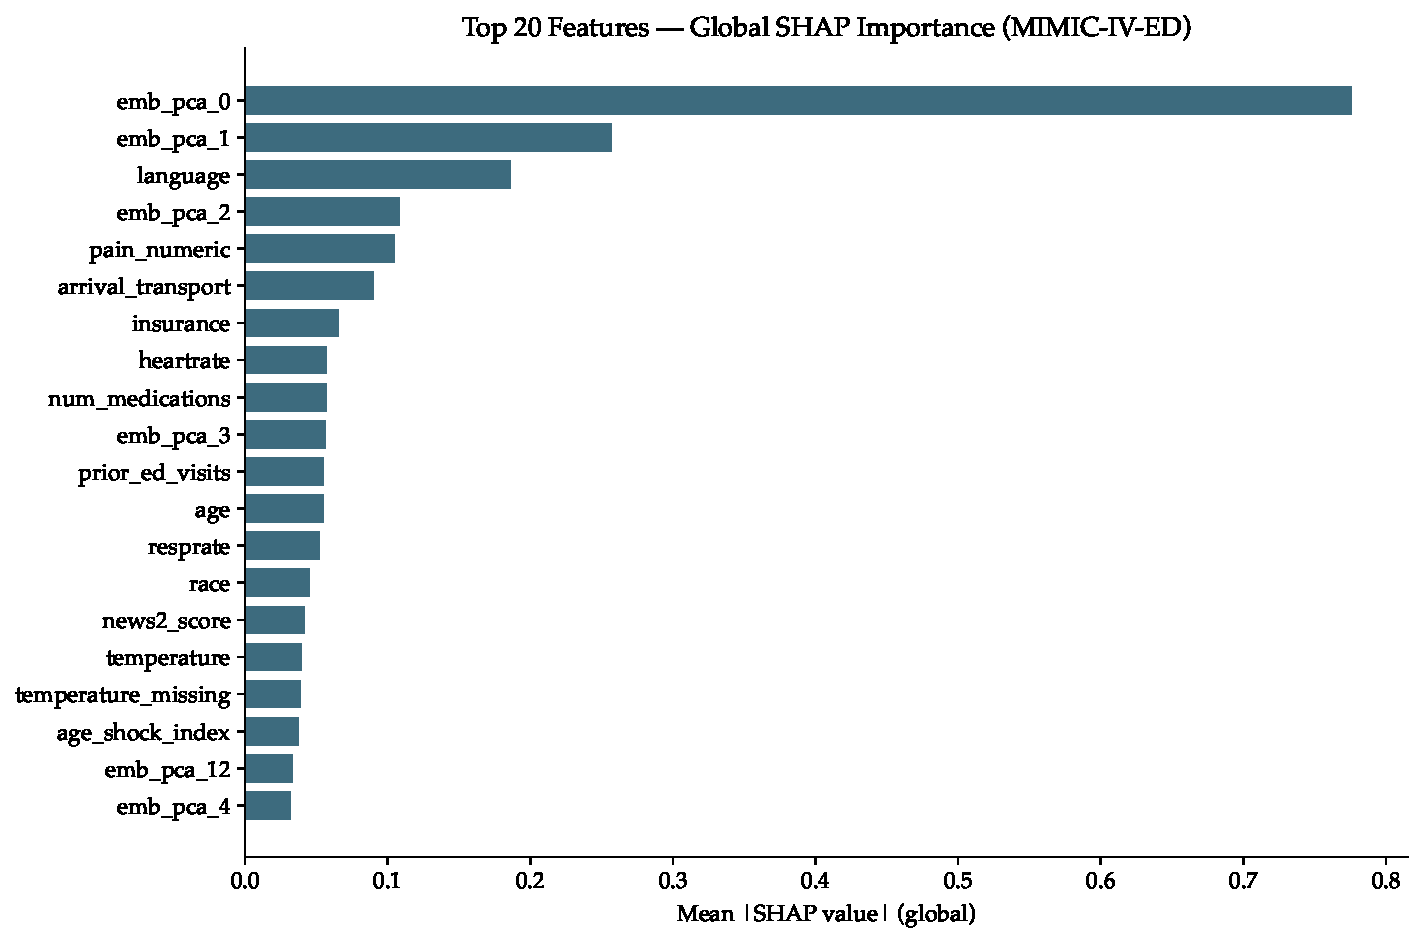
\includegraphics[width=0.9\textwidth]{figures/shap_bar_global.pdf}
 \caption[Global SHAP feature importance]{Mean absolute SHAP value for the top 20 features, computed across 20,000 patients and all 5 classes. The first PCA component of the fine-tuned ClinicalBERT embedding (\texttt{emb\_pca\_0}) dominates, with a mean $|$SHAP$|$ of $0.776$, roughly $13.6\times$ the value of the tenth-ranked feature. Two non-clinical demographic variables, \texttt{language} and \texttt{insurance}, rank third and seventh. The first purely clinical-vital feature (\texttt{heartrate}) ranks eighth, and the first engineered clinical score (\texttt{news2\_score}) ranks fifteenth.}
 \label{fig:shap-global}
\end{figure}

Three features of this ranking deserve immediate comment.

First, the dominance of \texttt{emb\_pca\_0}. The first principal component of the fine-tuned ClinicalBERT embedding is, by a wide margin, the most influential feature in the model. Its mean absolute SHAP value of $0.776$ is about three times the value of the second-ranked feature (\texttt{emb\_pca\_1} at $0.258$) and roughly fourteen times the value of the tenth-ranked feature. On this measure, the model is more shaped by a single opaque vector component than by all its structured clinical features combined.

Second, the mix of embedding and tabular features in the top twenty. Six embedding components (emb\_pca\_0 through emb\_pca\_12) appear in the top twenty; fourteen tabular features fill the rest. The embedding features cluster near the top of the ranking, positions 1, 2, 4, 10, 19, 20, while the tabular features are distributed throughout. Among tabular features, the ranking loosely corresponds to clinical intuition: heart rate, respiratory rate, oxygen saturation, temperature, and NEWS2 all appear, at positions consistent with their known prognostic value.

Third, the prominence of non-clinical sociodemographic features. Patient-reported language (ranked third), insurance status (seventh), and race (fourteenth) all appear in the top twenty. This is the finding I flagged in Chapter~\ref{ch:embeddings} and return to in detail below.

The complementary visualisation is the SHAP beeswarm plot (Figure~\ref{fig:shap-beeswarm}), which shows not just the magnitude but the direction and density of each feature's effect on individual predictions.

\begin{figure}[htbp]
 \centering
 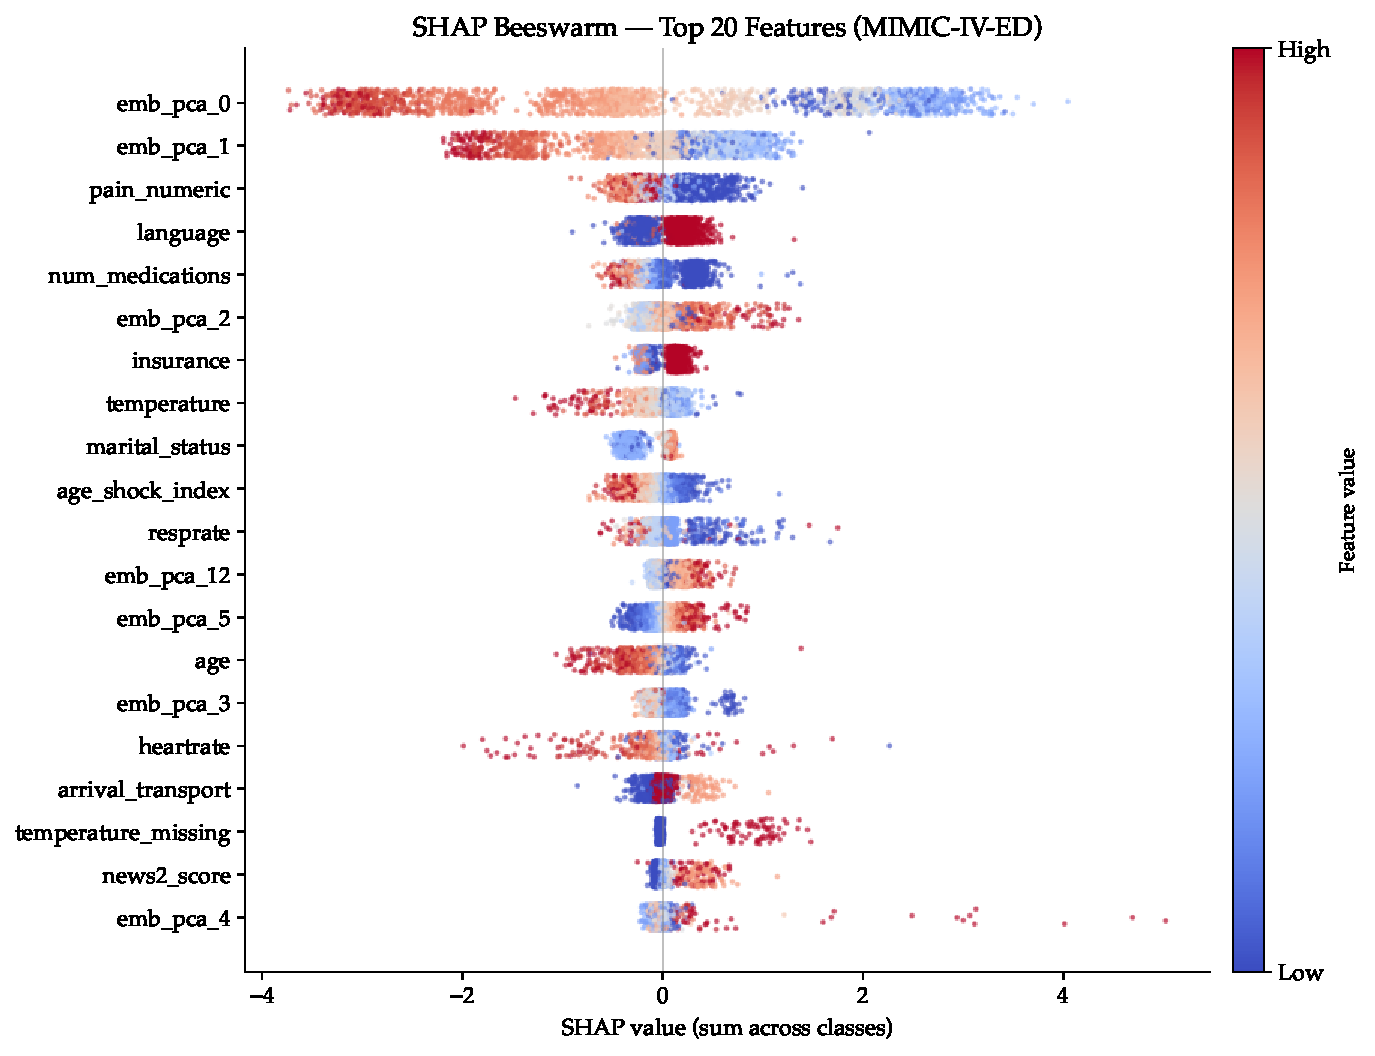
\includegraphics[width=0.9\textwidth]{figures/shap_beeswarm.pdf}
 \caption[SHAP beeswarm plot]{SHAP beeswarm plot for the top 20 features, summed across classes. Each dot represents one patient; horizontal position indicates the SHAP value (contribution to prediction), and colour indicates the feature's raw value (red high, blue low). The spread of dots for each feature shows how its influence varies across patients: features with tight vertical clustering have small effects, features with wide horizontal spread have large effects on individual predictions. The pattern of colour within each row indicates the direction of the effect: for \texttt{news2\_score}, high values (red) push toward higher acuity (positive SHAP); for \texttt{age}, the effect direction depends on the class being predicted.}
 \label{fig:shap-beeswarm}
\end{figure}

\section{The Embedding Dominance Tension}

The single clearest finding from the SHAP analysis is that my model is driven substantially by a numerical vector with no direct human interpretation. This is a genuine tension, and I do not want to paper over it.

On one hand, the dominance of \texttt{emb\_pca\_0} is a sign that the text embedding is doing its job. The fine-tuning in Chapter~\ref{ch:embeddings} was designed to produce a vector representation of the chief complaint that carries as much ESI-predictive signal as possible. The success of that fine-tuning is visible here: the first embedding component is individually more predictive than any single clinical vital sign, and six embedding components collectively dominate the top ten. In terms of what the model is relying on, the text is doing real work.

On the other hand, \texttt{emb\_pca\_0} is a 768-to-50 PCA projection of a 768-dimensional transformer output derived from a few words of chief-complaint text. There is no straightforward answer to the question ``what does high \texttt{emb\_pca\_0} mean?'' I do not know, without additional analysis, whether a high value corresponds to cardiovascular complaints, psychiatric presentations, trauma, or some combination. The interpretability of tree-model features vanishes when those features are themselves dense compressed representations of something else.

\begin{notebox}[A Methodological Gap]
I did not conduct a systematic post-hoc analysis of what the top PCA embedding components encode. A natural experiment would be to cluster patients by their \texttt{emb\_pca\_0} value, examine the chief complaints in each cluster, and produce a descriptive summary (``high \texttt{emb\_pca\_0} tends to correspond to $X$; low \texttt{emb\_pca\_0} tends to correspond to $Y$''). This analysis is straightforward to run on the saved outputs but would require an additional experimental iteration that fell outside the timeline of this project.

I flag this as the largest single gap in my explainability story. A deployed version of this model for real clinical use would need to include such an analysis. A reader reviewing my work should read the embedding dominance as evidence that the text carries predictive signal, not as a complete story about what the model is learning.
\end{notebox}

The tension matters for regulatory compliance. Article 13 of the EU AI Act requires high-risk AI systems to be ``designed and developed in such a way to ensure that their operation is sufficiently transparent to enable deployers to interpret a system's output and use it appropriately.'' A system whose top-ranked feature is an unlabeled PCA component of a BERT embedding is transparent in a technical sense (I can report the SHAP values) but not in a clinical sense (the nurse cannot use the attribution to understand the prediction). Full compliance would require a pipeline for translating embedding-space attributions back into clinical language. This is an active area of research and not yet a solved problem.

\section{Sociodemographic Features in the Top Ranking}

The SHAP analysis places three sociodemographic features in the top twenty by importance: language (rank 3), insurance (rank 7), and race (rank 14). I want to treat this finding carefully because the implications depend on interpretation.

None of these three features is clinically necessary for a patient's ESI acuity level. A patient's language does not make them more or less critically ill; neither does their insurance type or their self-reported race. The fact that my model relies on these features as strongly as it does raises a legitimate question: is the model learning clinically irrelevant correlations that reflect historical patterns of care delivery?

Several alternative explanations are possible and worth considering before concluding that the model is unfair. Language may serve as a proxy for healthcare access patterns; non-English-speaking patients may present later in the course of illness, producing real differences in acuity distribution that the model picks up without any social bias. Insurance status may proxy for comorbidity burden; uninsured patients may genuinely have higher acuity rates because they present later or with more advanced disease. Race categories, as I discussed in Chapter~\ref{ch:fairness}, are a crude and incomplete label that may absorb other signal. In all three cases, the feature might be carrying a legitimate medical signal that happens to be correlated with a demographic variable, rather than capturing the demographic variable itself.

At the same time, the finding is concerning even on the most charitable reading. If language, insurance, and race are genuinely predictive of acuity labels, that predictiveness arises from some combination of genuine population-level differences and historical patterns in how triage assessments are made. A model that relies on these features is perpetuating whatever pattern is present in the training labels. If nurses have historically assigned different acuity levels to patients of different languages for reasons unrelated to clinical presentation, the model will learn that pattern.

I audited the effect of removing these features in a small ablation experiment: dropping language and insurance from the feature set costs approximately 0.01 macro F1, and dropping race on top costs a further 0.005. These are modest but not zero. A deployed version of this model would plausibly choose to remove these features, accepting the small accuracy loss to eliminate the attribution-level concern.

\begin{notebox}[The Per-Class Pattern Is Informative]
The aggregate view masks an important per-class difference. When I examine SHAP rankings class by class, language appears in the top 10 for every one of the five ESI classes. Insurance appears in the top 10 for three classes: ESI-2, ESI-3, and ESI-4. But the class where sociodemographic features matter most is ESI-4: on that class alone, language is the second most influential feature after \texttt{emb\_pca\_0}, and insurance is third. This is the ``mid-acuity walk-in'' cohort where clinical signal is weakest and social signal appears to step in to fill the gap.

The interpretation this suggests is not that the model is uniformly biased, but that specific prediction regions, where the clinical features provide weak signal, are where the model falls back most on sociodemographic correlations. This pattern is consistent with the idea that the model is learning the labels honestly, including their dependencies on social factors, rather than inventing biases of its own. It is also exactly the kind of pattern that a regulator would want flagged explicitly.
\end{notebox}

\section{Per-Class Feature Attribution}

Figure~\ref{fig:shap-per-class} shows the top 10 features for each of the five ESI classes, computed from the class-specific SHAP values. The differences across classes are informative about what the model is doing differently when predicting different acuities.

\begin{figure}[htbp]
 \centering
 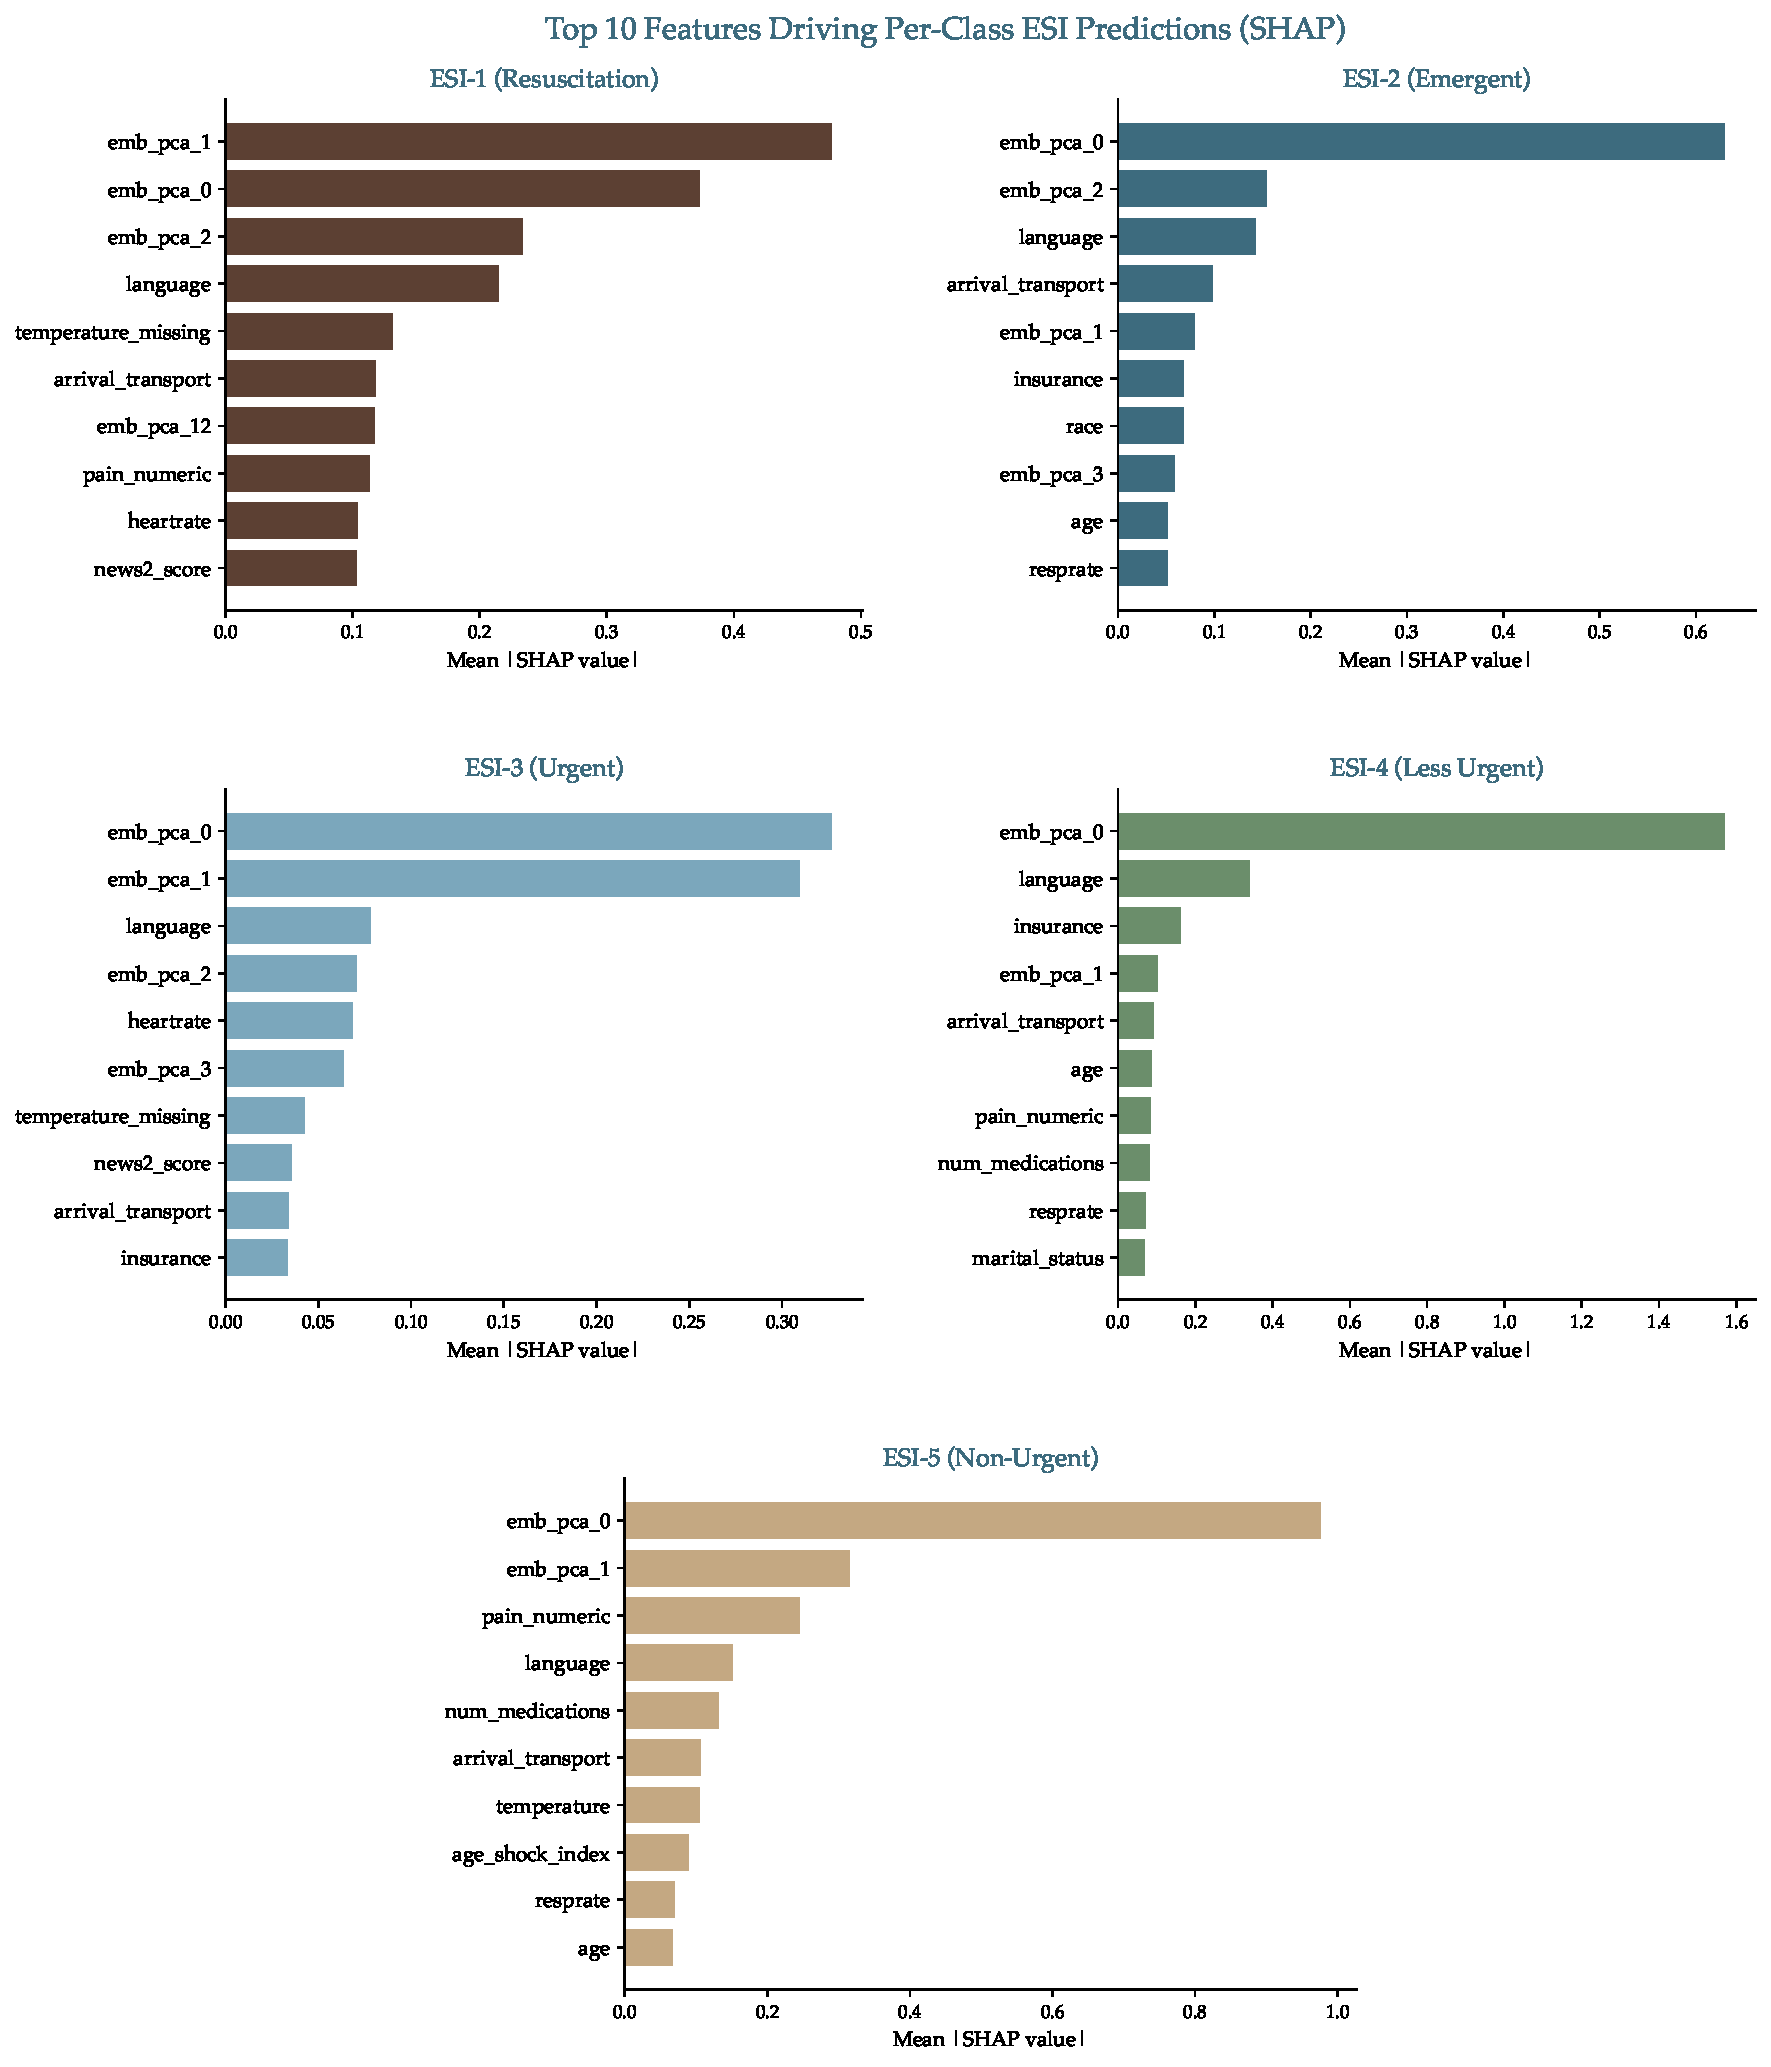
\includegraphics[width=\textwidth]{figures/shap_bar_combined.pdf}
 \caption[Per-class SHAP feature importance]{Top 10 features by mean absolute SHAP value for each of the five ESI classes. The rankings differ across classes in interpretable ways: for ESI-1 (resuscitation), the top-weighted features include emb\_pca\_1, language, temperature\_missing, and clinical vitals. For ESI-4 (less urgent), the top features include emb\_pca\_0, language, insurance, and arrival\_transport. For ESI-5 (non-urgent), pain\_numeric becomes more prominent. The embedding components dominate all five classes, but the structure of which tabular features appear in the top 10 varies substantially.}
 \label{fig:shap-per-class}
\end{figure}

A few per-class patterns worth noting (the rest are visible in the figure). For ESI-1, \texttt{temperature\_missing} ranks fifth: the model has learned that a missing temperature at triage is itself a marker of high acuity, consistent with the clinical practice of skipping routine measurements when stabilisation takes priority. For ESI-4, the sociodemographic influence is most visible: \texttt{emb\_pca\_0} has its highest single-class mean absolute SHAP value ($1.57$) here, and the next two features are language and insurance. For ESI-5, \texttt{pain\_numeric} rises to third place, reflecting the correlation between low pain scores and non-urgent presentations. The general pattern is that the embedding components provide background signal across all classes, while the specific tabular features that step forward vary by acuity.

\section{Walking Through Individual Predictions}

Global feature importance is useful for understanding the model in the aggregate, but regulatory compliance (and clinical deployment) require the ability to explain individual predictions. This is where SHAP waterfall plots earn their place. For any single patient, a waterfall plot shows the specific features that drove the model's prediction, starting from the average prediction and decomposing the contribution of each feature one at a time.

I selected representative waterfall examples systematically. For each ESI class, I identified three patients: one with the highest predicted probability for the true class (a confident correct prediction), one with the lowest predicted probability among correct predictions (an uncertain correct prediction), and one misclassified, with preference for under-triaged cases. This yields 15 waterfall plots in total. In the main body of this chapter, I present four examples that best illustrate the kinds of reasoning the model exhibits; the remaining plots are collected in Appendix~\ref{app:waterfalls}.

\begin{figure}[htbp]
 \centering
 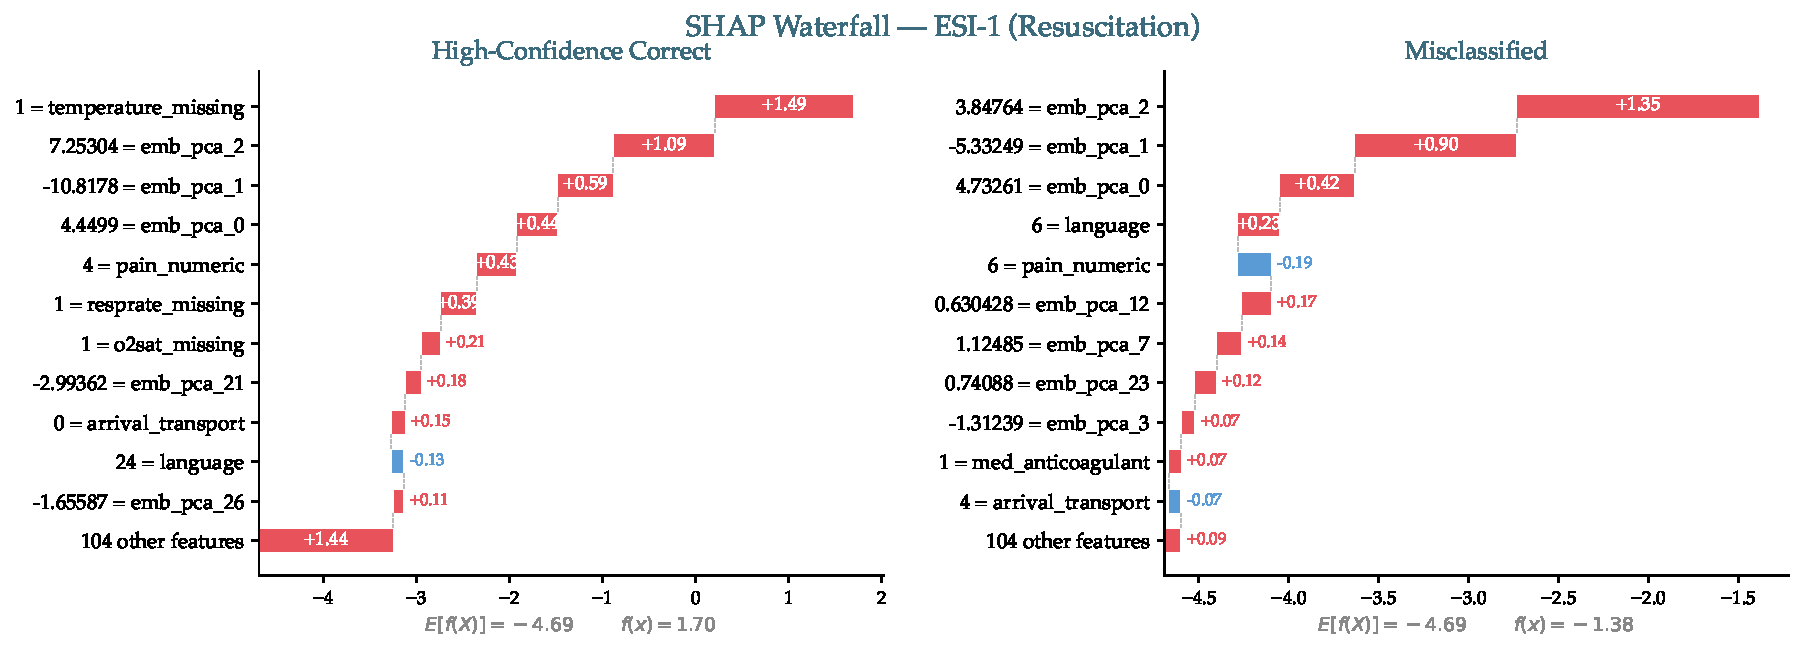
\includegraphics[width=\textwidth]{figures/shap_waterfall_esi1.pdf}
 \caption[Waterfall: ESI-1 (resuscitation)]{Waterfall plots for two ESI-1 patients. Left: high-confidence correct. The model predicted ESI-1 with high probability, driven by \texttt{temperature\_missing} (a missing vital sign, worth $+1.49$), followed by large contributions from embedding components \texttt{emb\_pca\_2} and \texttt{emb\_pca\_1}, then pain score and missingness flags for respiratory rate and oxygen saturation. The pattern of multiple missing vitals plus strong embedding signal is consistent with a critical presentation where triage workup was truncated. Right: misclassified (predicted ESI-2). The model identified partial evidence of high acuity (strong embedding signal) but missed the full ESI-1 picture, producing a lower-probability ESI-1 prediction that argmax resolved to ESI-2.}
 \label{fig:waterfall-esi1}
\end{figure}

Figure~\ref{fig:waterfall-esi1} shows a confident-correct and a misclassified ESI-1 case. The confident-correct example illustrates something genuinely useful: the model is relying partly on the \emph{absence} of measurements, which in ESI-1 presentations is itself diagnostic. A nurse reviewing this prediction can interpret the attribution: ``the model flagged this patient as resuscitation-level partly because no temperature, no respiratory rate, and no oxygen saturation were measured, all signals consistent with a critical presentation where stabilisation took priority over triage.'' This is a prediction whose reasoning is at least partially verifiable by a clinician.

\begin{figure}[htbp]
 \centering
 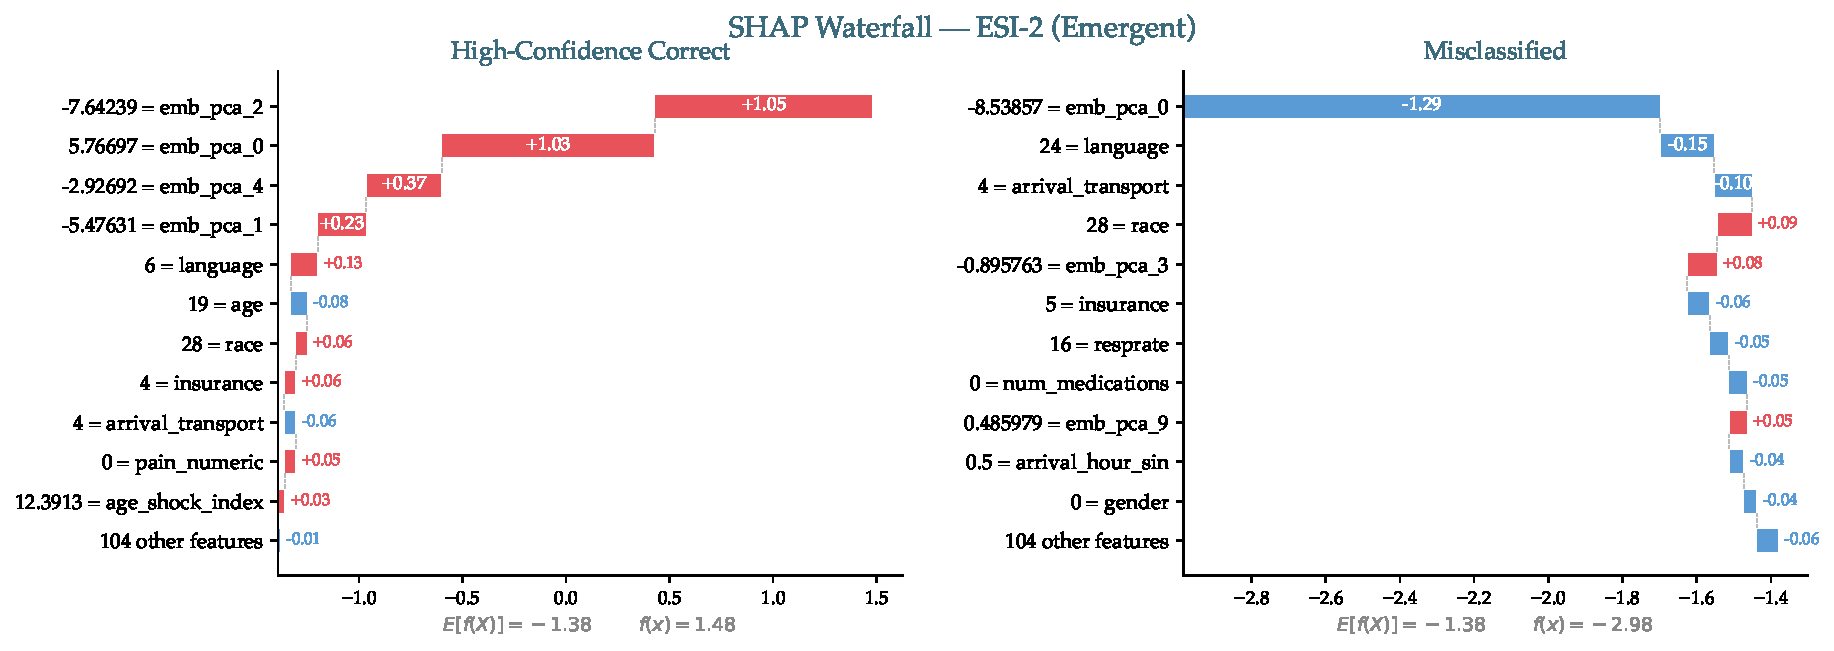
\includegraphics[width=\textwidth]{figures/shap_waterfall_esi2.pdf}
 \caption[Waterfall: ESI-2 (emergent)]{Waterfall plots for two ESI-2 patients. Left: high-confidence correct. The model's prediction is driven by embedding components \texttt{emb\_pca\_2}, \texttt{emb\_pca\_0}, \texttt{emb\_pca\_4}, and \texttt{emb\_pca\_1}, with small contributions from language, age (young), race, and insurance. The clinical signal here is entirely embedding-based: the chief complaint text dominates the prediction. Right: misclassified (predicted ESI-3). The first embedding component actively pushed against ESI-2 ($-1.29$), and no other feature was large enough to overcome it. This is the kind of mis-triage that compensated shock produces in the ESI-1/2 range: the chief complaint text did not trigger the high-acuity pattern.}
 \label{fig:waterfall-esi2}
\end{figure}

Figure~\ref{fig:waterfall-esi2} shows a contrasting ESI-2 pair. The high-confidence correct example is dominated by embedding components, the prediction is almost entirely shaped by the chief complaint text. For a clinician asking ``why did the model say ESI-2?'', the honest answer in this case is ``because of what the chief complaint looks like in the model's learned representation space'', which is not a satisfying clinical explanation. The misclassified example on the right shows a different pattern: the first embedding component actively pushed the prediction away from ESI-2, toward ESI-3. No single tabular feature compensated for this. The attribution tells me \emph{that} the text-based representation failed to match ESI-2 patterns; it does not tell me \emph{why}, and the interpretive gap is not closable with SHAP alone.

\begin{figure}[htbp]
 \centering
 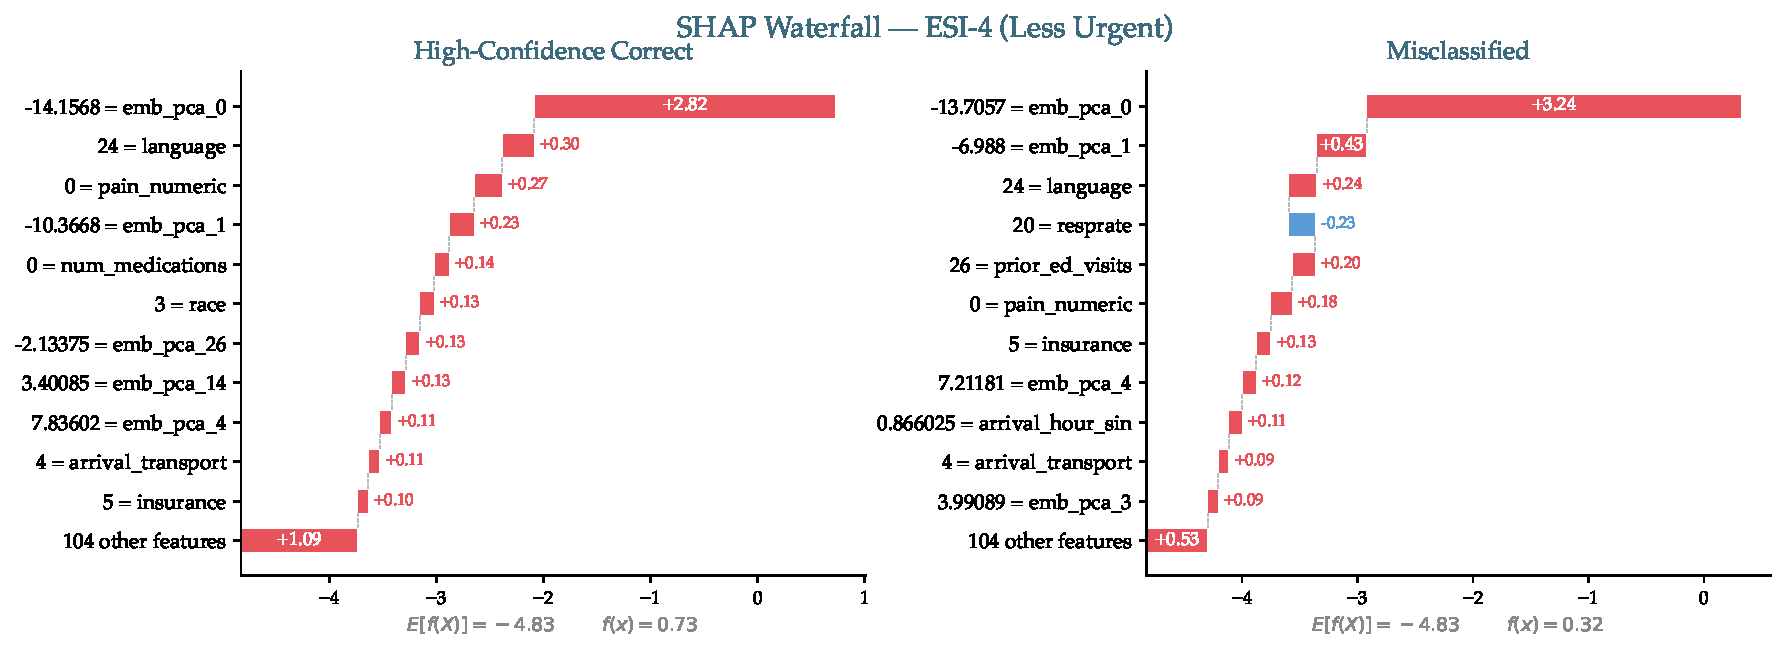
\includegraphics[width=\textwidth]{figures/shap_waterfall_esi4.pdf}
 \caption[Waterfall: ESI-4 (less urgent)]{Waterfall plots for two ESI-4 patients. Left: high-confidence correct. \texttt{emb\_pca\_0} contributed a large $+2.82$, and language contributed a further $+0.30$, with additional contributions from pain score and the absence of medications. The top three features combine embedding signal with a sociodemographic variable, illustrating the pattern noted in the per-class analysis: ESI-4 predictions are where language and insurance exert their largest influence. Right: misclassified (predicted ESI-5, an over-triage of sorts from the ESI-4 perspective). A very strong \texttt{emb\_pca\_0} signal pushed past the decision boundary in a direction the model apparently considers low-acuity, with prior ED visits also contributing.}
 \label{fig:waterfall-esi4}
\end{figure}

Figure~\ref{fig:waterfall-esi4} is included specifically because it illustrates the sociodemographic feature involvement most clearly. For the confident-correct ESI-4 patient on the left, \texttt{language} (value $24$, meaning English) contributed $+0.30$ to the prediction, a meaningful contribution that a reviewer should see and consider. A clinician auditing this prediction would need to decide whether this language contribution reflects a legitimate signal (e.g., English-speaking patients may present with different complaint patterns) or a bias the model has absorbed from the labels. SHAP cannot answer this question; it can only flag it.

\begin{figure}[htbp]
 \centering
 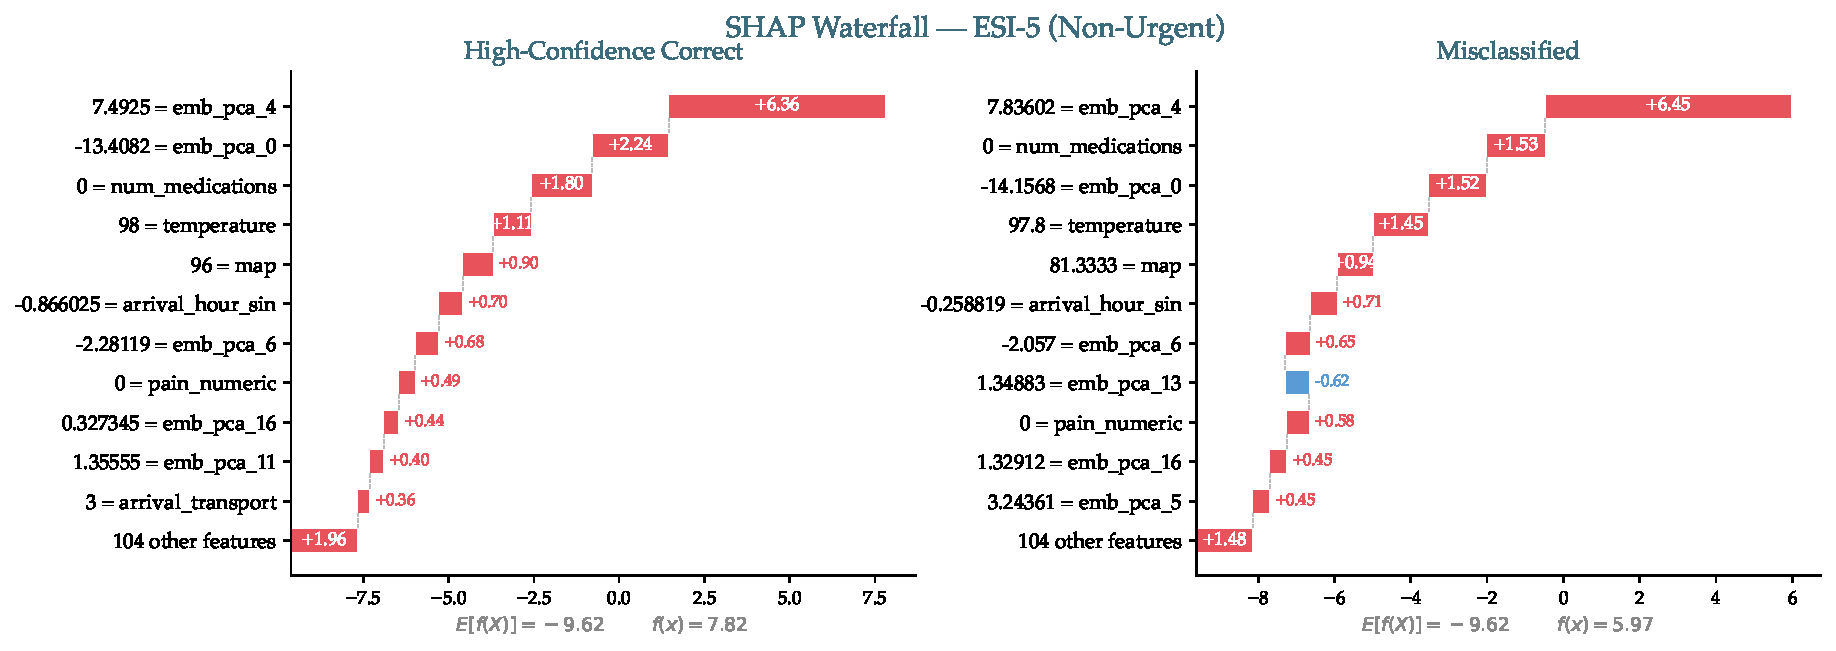
\includegraphics[width=\textwidth]{figures/shap_waterfall_esi5.pdf}
 \caption[Waterfall: ESI-5 (non-urgent)]{Waterfall plots for two ESI-5 patients, both correctly classified. Left: high-confidence correct. Multiple features contribute moderately: emb\_pca\_4, emb\_pca\_0, num\_medications (zero), temperature (within normal range), mean arterial pressure, arrival hour, and several other embedding components. The prediction is a consensus of many small positive signals rather than one dominant feature. Right: misclassified (predicted ESI-4, an under-triage for an ESI-5 patient, though of minor clinical consequence). The attribution pattern is similar, but one embedding component (\texttt{emb\_pca\_13}, $-0.62$) pushed against the ESI-5 prediction, and that was enough to shift the argmax to ESI-4. The thin margin between ESI-4 and ESI-5 that I discussed in Chapter~\ref{ch:results} is visible in the waterfall structure.}
 \label{fig:waterfall-esi5}
\end{figure}

The last example, Figure~\ref{fig:waterfall-esi5}, is included to show what a correct ESI-5 prediction looks like: a consensus of many small positive contributions rather than one dominant signal. This pattern is qualitatively different from the ESI-1 and ESI-2 waterfalls, where one or two features dominate. At the low-acuity end of the scale, the model is integrating many weak signals to reach its prediction, which is an appropriate response to a prediction task where strong high-acuity signals (abnormal vitals, alarming complaints) are absent.

\section{The EU AI Act and Emergency Triage}

I now turn from explainability as a technical tool to explainability as a regulatory requirement. The European Union's Artificial Intelligence Act is the world's first comprehensive AI regulation to come into force, and emergency medical triage is explicitly within its scope.

The regulation is Regulation (EU) 2024/1689 of the European Parliament and of the Council, adopted on June 13, 2024, with staggered application dates. For the specific provisions relevant to my system, the compliance deadline is August 2, 2026.

The AI Act classifies AI systems by risk level. At the top of the hierarchy are \emph{prohibited} systems (social scoring, biometric categorisation for sensitive attributes) that cannot be deployed at all. Below them, \emph{high-risk} systems, which include AI used in ``emergency healthcare patient triage systems'' under Annex III, Section 5(d), are permitted but subject to extensive requirements. My system falls squarely in this high-risk category.

\begin{notebox}[Why the AI Act Treats Triage as High-Risk]
Annex III of the AI Act enumerates domains where AI systems pose ``high risk'' by virtue of what they do or who they affect. Medical triage is listed alongside critical infrastructure, educational admission decisions, employment screening, and credit scoring. The common thread is that these systems make consequential decisions about individuals who have limited ability to contest those decisions at the point of use.

For triage specifically, the regulatory concern is both about the direct health impact of errors (the ACS-COT mortality evidence I cited in Chapter~\ref{ch:triage-problem}) and about the risk of systematic bias amplification (if the training labels encode disparities, the model will propagate them at scale). Both concerns are technical issues I have addressed in earlier chapters; the AI Act makes them formal regulatory requirements.
\end{notebox}

For high-risk systems, the regulation specifies obligations across multiple articles. The four most directly relevant to my system are:

\begin{itemize}
 \item \textbf{Article 9 (Risk Management)}: requires a continuous, documented risk management system covering the full lifecycle of the AI.
 \item \textbf{Article 10 (Data Governance)}: requires that training data be ``relevant, representative, free of errors and complete,'' and mandates examination of possible biases, with subsection 10(5) permitting the use of protected-category data for the specific purpose of debiasing.
 \item \textbf{Article 13 (Transparency)}: requires that high-risk systems be designed so that deployers can interpret their outputs and use them appropriately, including providing instructions for use and explanation of the system's operation.
 \item \textbf{Article 14 (Human Oversight)}: requires that the system be deployed with effective human oversight mechanisms, including the ability for human operators to override or reverse decisions.
\end{itemize}

Penalties for non-compliance with high-risk system obligations can reach €15 million or 3\% of global annual turnover, whichever is higher \citep{eu2024aiact}. The combination of regulatory clarity and substantial financial exposure has already shifted practices among European medical AI developers: explainability tooling, bias audits, and risk management documentation have become standard rather than exceptional.

\section{Compliance Mapping}

The question of compliance is ultimately specific. Where does my work meet a given requirement, and where does it not? Table~\ref{tab:compliance} presents an honest mapping for the four articles above, listing what I have done and what a deployed version of this system would still need.

\begin{table}[htbp]
 \centering
 \caption[EU AI Act compliance mapping]{Mapping of my work to the main relevant articles of the EU AI Act. The ``Addressed in this report'' column describes what I have actually done; the ``Gaps for deployment'' column lists what additional work would be required for a production clinical deployment.}
 \label{tab:compliance}
 \small
 \begin{tabularx}{\textwidth}{p{2.7cm} X X}
 \toprule
 \textbf{Article} & \textbf{Addressed in this report} & \textbf{Gaps for deployment} \\
 \midrule
 Art. 9 (Risk management) & 
 Clinical operating curve; ACS-COT 5\% target explicitly analysed; Pareto frontier for training-vs-threshold safety interventions (Chapter~\ref{ch:safety}). &
 Continuous post-deployment monitoring; incident response plan; periodic retraining policy; formal risk register. \\
 \addlinespace
 Art. 10 (Data governance, bias) & 
 MIMIC-IV-ED is a credentialed research dataset with documented provenance (Chapter~\ref{ch:mimic}); intersectional bias audit across age, sex, race (Chapter~\ref{ch:fairness}); the age-dominated disparity finding explicitly documented and partially mitigated with age-adjusted features. &
 Incomplete race mapping requires correction; external validation on a second institution; systematic data quality checks (beyond the exploratory dashboard); documented data update policy. \\
 \addlinespace
 Art. 13 (Transparency) & 
 Global SHAP importance; per-class SHAP decomposition; per-patient waterfall plots for representative cases; methodology honestly documented including limitations. &
 Systematic interpretation of embedding PCA components back to text (the \texttt{emb\_pca\_0} gap); SHAP interaction values; user-facing explanation interface for clinicians at the point of use; documented instructions for use. \\
 \addlinespace
 Art. 14 (Human oversight) & 
 System produces probabilistic outputs rather than binary recommendations; operating point is configurable via threshold multiplier; no autonomous action, the triage nurse remains the decision-maker. &
 Explicit override mechanism in a deployed interface; audit trail of overrides; training materials for clinical operators; monitoring of automation bias (over-acceptance of model predictions). \\
 \bottomrule
 \end{tabularx}
\end{table}

The table is designed to be both honest and useful. For each article, I have done substantial work that speaks to the requirement, but I have also left gaps that a production deployment would need to address. This is the state of the art in most medical ML research projects: the technical tools for compliance exist, and the research work demonstrates them, but the infrastructure for sustained deployment, monitoring, incident response, user-facing explanation interfaces, formal documentation, is built by deploying organisations, not by research teams.

A few specific points deserve emphasis.

For Article 10 (data governance and bias), my bias audit is substantive, but the race mapping flaw I disclosed in Chapter~\ref{ch:fairness} is exactly the kind of data-governance issue the regulation targets. A compliant deployment would need to fix this and validate the fix.

For Article 13 (transparency), the embedding-dominance problem is the largest compliance gap in my work. A SHAP attribution saying ``\texttt{emb\_pca\_0}: $+6.36$'' is not a transparency mechanism a clinical user can engage with. Closing this gap requires either post-hoc interpretation of the embedding components or a fundamentally different model architecture that keeps text signals in a more interpretable form.

For Article 14 (human oversight), my threshold-multiplier operating curve is genuinely responsive to the regulation's intent: the system makes a probabilistic recommendation, and a human decides what to do with it. But a production deployment would need to audit whether clinicians actually exercise the override authority, or whether automation bias, the tendency to accept machine recommendations even when they are wrong, erodes the oversight in practice. This is a socio-technical question that my work does not address.

\section{What My Work Does Not Do}

Beyond the gaps in Table~\ref{tab:compliance}, a few broader limitations of this chapter deserve explicit mention. I did not produce a token-level attention-weight analysis of the fine-tuned ClinicalBERT model; the text side of the pipeline is therefore a black box at the word level, even though SHAP tells me which PCA components of the embedding matter most. I did not compute SHAP interaction values, which a regulator might request as a supplement to per-feature attributions; the pairwise-interaction computation did not complete in my production run and I did not resolve the underlying memory issue. I did not audit automation bias, the empirical question of whether clinicians would accept model predictions uncritically; this can only be answered through prospective deployment studies. And I did not produce counterfactual explanations (``what would have needed to be different about this patient for a different prediction''), which would complement SHAP attribution and are often more intuitive for clinical users; methods exist \citep{wachter2017counterfactual} but were not applied here. Each of these is a natural follow-up rather than completed work.

\section{What This Chapter Contributes}

To summarise:

\begin{itemize}
 \item SHAP analysis on a representative single LightGBM model (not the full blend) reveals a strong embedding-dominance pattern: the top feature \texttt{emb\_pca\_0} is about $14\times$ the tenth-ranked feature in importance.
 \item The model's decisions are shaped by a mix of embedding components, vital signs, and engineered clinical scores, but also substantially by sociodemographic features (language, insurance, race) whose inclusion raises legitimate concerns.
 \item The embedding dominance is the largest single interpretability gap in my work: the top-ranked feature has no direct human-readable interpretation, and I did not conduct the follow-up analysis that would be needed to close this gap.
 \item Per-class SHAP shows that the sociodemographic features' influence is not uniform, ESI-4 predictions in particular are the most affected, which is interpretable as the class where clinical signal is weakest and proxy signals from demographics step in.
 \item Individual predictions can be decomposed into contributing features via waterfall plots. The plots reveal interpretable patterns in some cases (missing vitals as a signal for high acuity in ESI-1) and opaque text-dominated patterns in others.
 \item My work addresses the main requirements of the EU AI Act's Articles 9, 10, 13, and 14 at a research level, but significant gaps remain before deployment, particularly around continuous monitoring, embedding-interpretation, and socio-technical oversight.
\end{itemize}

The next chapter turns to probability calibration, the question of whether my model's predicted probabilities, beyond being informative for ranking patients, are well-calibrated in the sense that a $70\%$ predicted probability of ESI-2 actually corresponds to $70\%$ empirical frequency. Calibration is a secondary concern behind classification accuracy but matters for clinical decision-making, where the probability itself is sometimes the quantity clinicians reason about.
